\newchapter{Musket Ball: DM Implications}{Musket Ball Cluster: Dark Matter Implications}{Musket Ball Cluster: Dark Matter Implications}
\label{chapter:4}

\noindent Portions of this chapter were originally published in the article titled \emph{Discovery of a Dissociative Galaxy Cluster Merger with Large Physical Separation} which was published in the March 2012 issue of the Astrophysical Journal Letters (Volume 747, pp. L42). \\

Chapter abstract text

\section{Introduction}



Intro text \citep{Dawson:2012dl}

\section{Location Estimation}
For the original work of \citet{Dawson:2012dl} (see Chapter 2) I estimated the weak lensing subcluster positions and errors on their positions by using the location of the peak signal in a region and estimated the variance on the peak by measuring the peak location of each bootstrap iteration within the selected region.  
For this chapter, rather than using the location of the peak and variance of the peak, I have adopted an iterative centroid estimation scheme, similar to \citet{Randall:2008hs}. 
I begin by calculating the centroid of a large aperture that encompasses one subcluster, but excludes the other.
I then decrease the aperture, recenter on the previously calculated centroid, and estimate the centroid of the new aperture.
This process is repeated until the aperture is decreased to a radius of XXX kpc.
To estimate the uncertainty on the location I perform this process on each iteration of a random bootstrap sample map, resulting in a array of centroid values.
 The uncertainty on the location is then inferred from the variance of this array of centroid values.


\subsection{Galaxies}

\subsubsection{Noise and Systematic Effects}

\subsection{Gas}

\subsection{Weak Lensing}


\section{Gas--Weak Lensing Offset}

%copied from \citep{Dawson:2012dl}
Given the evident merger scenario we are able to use the first method of \citet{Markevitch:2004dl} and place a rough limit on the DM self-interaction cross-section, $\sigma_{\rm DM}$.
This method compares the scattering depth of the dark matter, $\tau_{\rm DM}=\sigma_{\rm DM}m^{-1}_{\rm DM} \Sigma_{\rm DM}$, with that of the ICM gas, $\tau_{\rm ICM}\approx 1$, where $m_{\rm DM}$ is the DM particle mass and $\Sigma_{\rm DM}$ is the surface mass density of the DM particles.
$\Sigma_{\rm DM}$ is approximately the WL measured surface mass density, $\Sigma$, since $\sim80\%$ of a typical cluster's mass is DM \citep{Diaferio:2008js}.
For ease of comparison with the results of \citet{Markevitch:2004dl} and \citet{Merten:2011gu} we examine the surface density averaged over the face of the subcluster within $r$=125\,kpc, which is $\Sigma\approx0.15$\,g\,cm$^{-2}$; thus we find $\sigma_{\rm DM} m_{\rm DM}^{-1} \lesssim 7$\,cm$^2$\,g$^{-1}$.  
Note that we cannot apply the velocity-dependent $\sigma_{\rm DM}$ constraint methods outlined by \citet{Markevitch:2004dl} since our analytic model assumes $\sigma_{\rm DM}$\,=\,0 \citep{Dawson:2012dl, Dawson:2012ub}.

\begin{figure}
%\plottwo{fig3a.eps}{fig3b.eps}
\plotone{Chapter2/fig3.png}
\caption[Comparison of the Subaru $i'$-band ground-based and HST space-based WL mass signal-to-noise maps of DLSCL J0916.2+2951 with the X-ray distribution and galaxy number density.]{Comparison of the Subaru $i'$-band ground-based (left) and HST space-based (right) WL mass signal-to-noise maps (color) of DLSCL J0916.2+2951 with the X-ray distribution (bold black contours) and galaxy number density (white contours, same as Figure \ref{fig2}). The peak centers and corresponding one sigma errors are denoted by the gray cross-hairs.
In both analyses there is agreement between the location and relative magnitude of galaxies and WL yet the majority of the cluster gas is centered $\sim1.4\arcmin$ between the North and South subclusters in a local mass underdensity, providing evidence that the North and South subclusters have undergone the first pass-through of a major merger.
The scale of each map is equivalent and the image field-of-view is the same as Figures \ref{fig1} \& \ref{fig2}.
The map created from the joint Subaru/HST catalog looks nearly identical to the HST map, with only slight variations in the scale (see Table \ref{tbl1}).
\label{fig3}}
\end{figure}

\section{Galaxy--Weak Lensing Offset}

Section text

%-----------------------------Figure Start------------------------------
% Single panel figure
\begin{figure}[t]
	\centering
	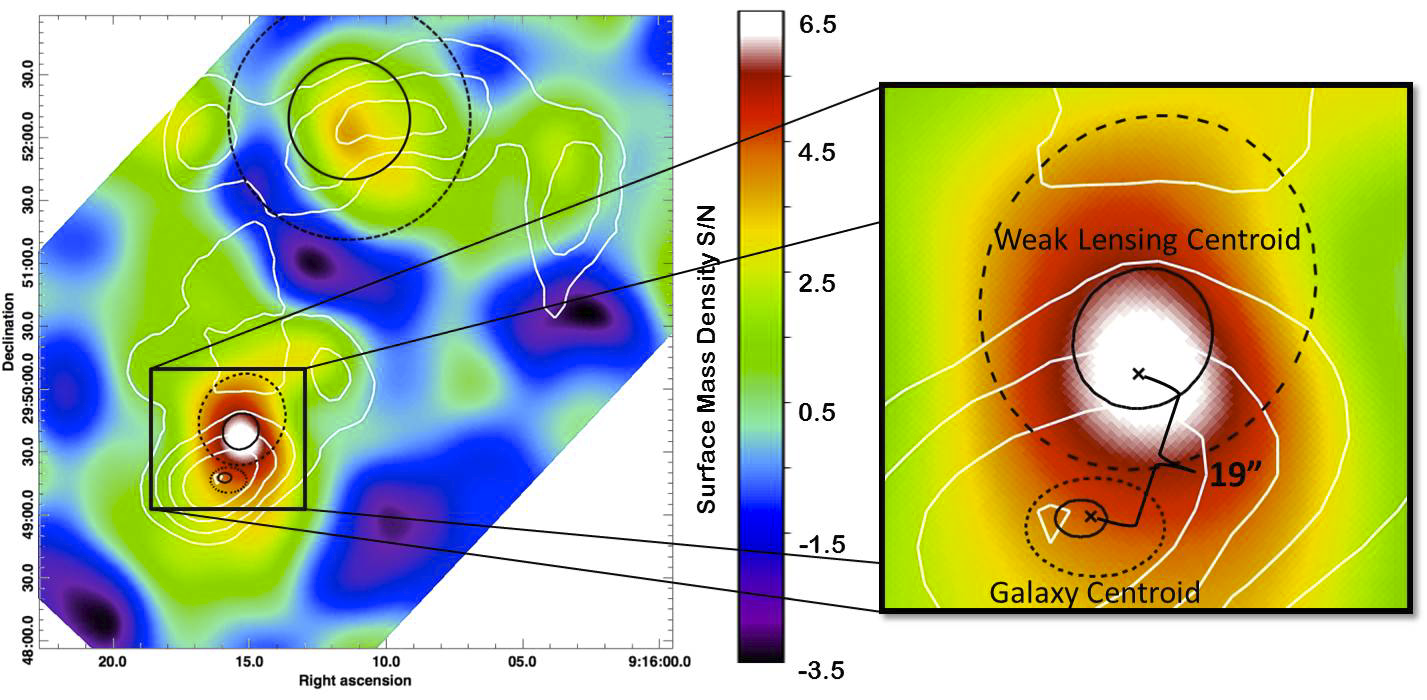
\includegraphics[width=6in]{Chapter4/WLgalaxyoffset.png}
	\caption[Musket Ball Cluster galaxy-weak lensing offset.]{
		\small{The WL mass signal-to-noise map based on HST measured shapes is shown in color with the galaxy number density isopleths in white.  
		The inset shows the 68\% (solid black) and 95\% (dashed black) confidence intervals on the South subcluster's WL and galaxy density centroids.  
		We have detected a 19" offset between the galaxies and the WL mass in the South subcluster that is consistent with the offset expected if DM has a non-zero cross-section just below the current published upper limits.  
		This is the best astrophysical evidence to date of a non-zero DM cross-section.  While a consistent offset is observed for the North subcluster, the large WL centroid error prohibits measurement of a significant offset for that subcluster.
		}
	}
	\label{fig2}
\end{figure}
%-----------------------------Figure End--------------------------------


\subsubsection{Noise and Systematic effects}

\textit{Copied from Chandra/HST proposal. Need to edit.}

Several sources of noise and systematic effect could cause such an offset:
(1) the mass of the northern subcluster pulling off the overall mass
centroid; (2) the gas mass just to the north doing the same; and (3)
unrelated structures along the line of sight. We show below that (2)
is the primary concern and can be solved with Chandra data, and that
(4) HST data are required to tighten up the statistical uncertainty on
the size of offset.  Together, these data will enable measurement of
$\sigma_{\rm DM}m_{\rm DM}^{-1}$.

\textbf{(1)} We model the surface mass density of the north and south subclusters with three NFW halos using masses determined by \citet{Dawson:2012dl}. We recursively estimate the centroid of this model and find an offset $3.4''$ from the true centroid towards the northern subcluster. 
\textbf{(2)} We then combine estimated surface mass densities of the
Central and South gas concentrations with the previous DM surface
densities from step (1) which results in a $7.6''$ centroid offset (dashed red curve of Figure \ref{fig3}).  
For perspective, if we double the gas mass the total offset increases to $10''$, or if we account for the uncertainty in our distribution of the gas mass the modeled centroid offset ranges from $3.4''$ to $9.4''$ (light red region of Figure \ref{fig3}). 
With the proposed Chandra observations we can better constrain the gas mass by approximately a factor of 10 and constrain the distribution of the gas mass so that the resulting uncertainty in the modeled centroid offset is reduced by at least a factor of 2 (dark red region of Figure \ref{fig3}).
\textbf{(3)} As discussed in \citet{Dawson:2012dl} we find no evidence of significant line of sight structures using our full sample of 654 spectroscopic redshifts (with uniform selection over $0<z<1.0$) as well as photometric redshifts. 
Based our findings we confidently rule out any line of sight structures with $M_{\rm 200}\gtrsim1\times10^{12} M_\odot$; any undetected structure will have negligible impact on the offset.
\textbf{(4)} We estimate the noise of the galaxy density and weak lensing centroids by performing the recursive centroid analysis on bootstrap samples of each.
For the galaxy density centroid errors we take 1000 bootstrap samples of the spectroscopically confirmed cluster galaxies and remaining galaxies with $0.43<z_{\rm phot}<0.63$ (roughly the cluster redshift $\pm\sigma_{z_{\rm phot}}$).
Similarly we estimate the weak lensing centroid errors by analyzing 1000 bootstrap samples of the lensed background galaxies.

\section{Discussion}

Discussion text

\subsection{Subsection title}

\section{Conclusions}

Conclusion text

\textbf{acknowledgements:}
Acknowledgment text
%\end{acknowledgements}

%\bibliographystyle{apj}
%\bibliography{Chapter1/chapter1}{}



%% The References
%\bibliographystyle{thesis}
%\begin{singlespacing}
%  \bibliography{Chapter3/chapter3}
%\end{singlespacing}
